
This suite of tools satisfies the necessities (i)~to search the OEIS offline
and to automate searches, (ii)~to work in the console and with notebooks and
(iii)~to have an unified working environment where a single, general purpose,
programming language is used to integrate the OEIS with a symbolic algebra
system. Here, \textit{Python} plays the role of the glue language, relying
on the module \textit{Sympy} for symbolic computations.

\section{The Crawler}

The script \verb|crawling.py| fetches sequences recursively where the union of
cross refs sections defines the fringe to fetch.  It features no threads, no
race conditions, no data sync; on the contrary, it lies on \textit{async/await}
Python primitives only for pure asynchronous computation and the implementation
boils down to $300$ lines of Python code.  In the end, it allows us to cache
portions of the OEIS to speed up repeated lookups and to restart from the cache
already fetched.

The script presents a help message to explain itself:
\VerbatimInput[fontsize=\small]{OEIS/crawler-help.txt}

We illustrate a typical session where we start from scratch; first of all, we
download two important and nice sequences, namely those corresponding to the
Fibonacci and Catalan numbers, respectively:
\VerbatimInput[fontsize=\small]{OEIS/crawler-fetching-command.txt}
we check the content of our cache with
\VerbatimInput[fontsize=\small]{OEIS/crawler-status.txt}
and display raw data displaying pure \textit{json} content about
the sequence $A000045$, using a simple printer provided by the Python module
\verb|json.tool|:
\VerbatimInput[fontsize=\small]{OEIS/crawler-A000045-chunk.txt}
Moreover, we can restart our downloading process from where we left before
\VerbatimInput[fontsize=\small]{OEIS/crawler-restarting.txt}
checking that new sequences are actually saved
\begin{Verbatim}[fontsize=\small]
$ python3.6 crawling.py
50 sequences in cache ./fetched/
354 sequences in fringe for restarting
\end{Verbatim}


Our implementation takes strong inspiration from
\citep{VANROSSUM:DAVIS:async:await}: the \verb|reader| class has the
responsibility to wait asynchronously for incoming data the \verb|read|
coroutine,
\inputminted[fontsize=\small,stripnl=false,firstline=28,lastline=39]
    {python}{deps/oeis-tools/src/crawling.py}

The \verb|fetcher| class has the responsibilities to (i)~create a socket with
OEIS server, (ii)~establish a working connection, (iii)~send an http
\verb|GET| request for the desired sequence, (iv)~wait for the fetching process
completes and (v)~close the socket and signal that the work ends
successfully.
\inputminted[fontsize=\small,stripnl=false,firstline=41,lastline=86]
    {python}{deps/oeis-tools/src/crawling.py}

The \verb|crawler| class has the responsibilities
(i)~to keeps a queue of task, one for each candidate sequence,
(ii)~to put each ready task into a scheduling process to get executed and
(iii)~to reclaim memory from completed task and to deque them.
\inputminted[fontsize=\small,stripnl=false,firstline=89,lastline=117]
    {python}{deps/oeis-tools/src/crawling.py}

Finally, the function \verb|oeis| puts all together and it is the main
interface exported by the \verb|crawling| module:
\inputminted[fontsize=\small,stripnl=false,firstline=195,lastline=221]
    {python}{deps/oeis-tools/src/crawling.py}

\section{The (Pretty) Printer}

The script \verb|pprinting.py| provides a proxy for searching in the OEIS, it
shows exactly the same content you get from usual search interface on
http://oeis.org; additionally, it provides (i)~tabular representation of
\verb|data| sections in \textit{one and two dimensions} using list and matrix
notation, respectively, (ii)~filtering capabilities on most result's sections
and (iii)~takes advantage of cached sequences built by the crawler.

The script presents a help message to explain itself:
\VerbatimInput[fontsize=\small]{OEIS/pprinting-help.txt}

\VerbatimInput[fontsize=\small]{OEIS/pprinting-A000045.txt}

The following command pretty prints (i)~the first 3 results from cached
sequences, (ii)~ranking them according to the most recent access time,
(iii)~reporting data only and (iv)~limiting up to 10 elements for linear
sequences:
\VerbatimInput[fontsize=\small]{OEIS/pprinting-data-only.txt}

\VerbatimInput[fontsize=\small]{OEIS/pprinting-pascal-matrix.txt}

\section{The Grapher}

The script \verb|graphing.py| allows us to represent networks where vertices
are sequences and edges are connections among them, according to \verb|xref|
sections in their json encoding. It integrates with the crawler tool by parsing
fetched json files and creating \verb|Graph| objects defined in the Python
module \verb|networkx|, then it provides a set of layouts to draw the graphs.

It presents a help message to explain itself:
\VerbatimInput[fontsize=\small]{OEIS/graphing-help.txt}

With the following command we can draw a graph that emphasises vertices
according to the number of \textit{incoming} connections, the aim here is to
show the most known sequences,
\begin{Verbatim}[fontsize=\small]
$ python3.6 graphing.py --layout FRUCHTERMAN-REINGOLD graph.png
\end{Verbatim}
and Figure \ref{fig:oeis:sequences:network} reports the graph.

Moreover, it can export essential data, such as the list of vertices and edges,
to build graphs using third-party software tools; in particular, libraries
using the \textit{Javascript} programming language are very powerful to solve
this task and we use the \verb|arborjs| library (freely available at
\url{http://arborjs.org/}) to display two additional graphs.

In Figure \ref{fig:oeis:sequences:network:fibonacci:catalan} we report again an
unlabeled network that shows the underlying structure of connections; on the
other hand, in Figure
\ref{fig:oeis:sequences:network:fibonacci:catalan:labeled} we add labels to
vertices in order to find the two main referenced vertices, that corresponds to
\textit{Fibonacci} and \textit{Catalan} numbers, respectively -- for the sake
of clarity, these graphs corresponds to a tiny subset of the entire
encyclopedia only, the more we fetch the more graphs get complex.

\begin{figure}
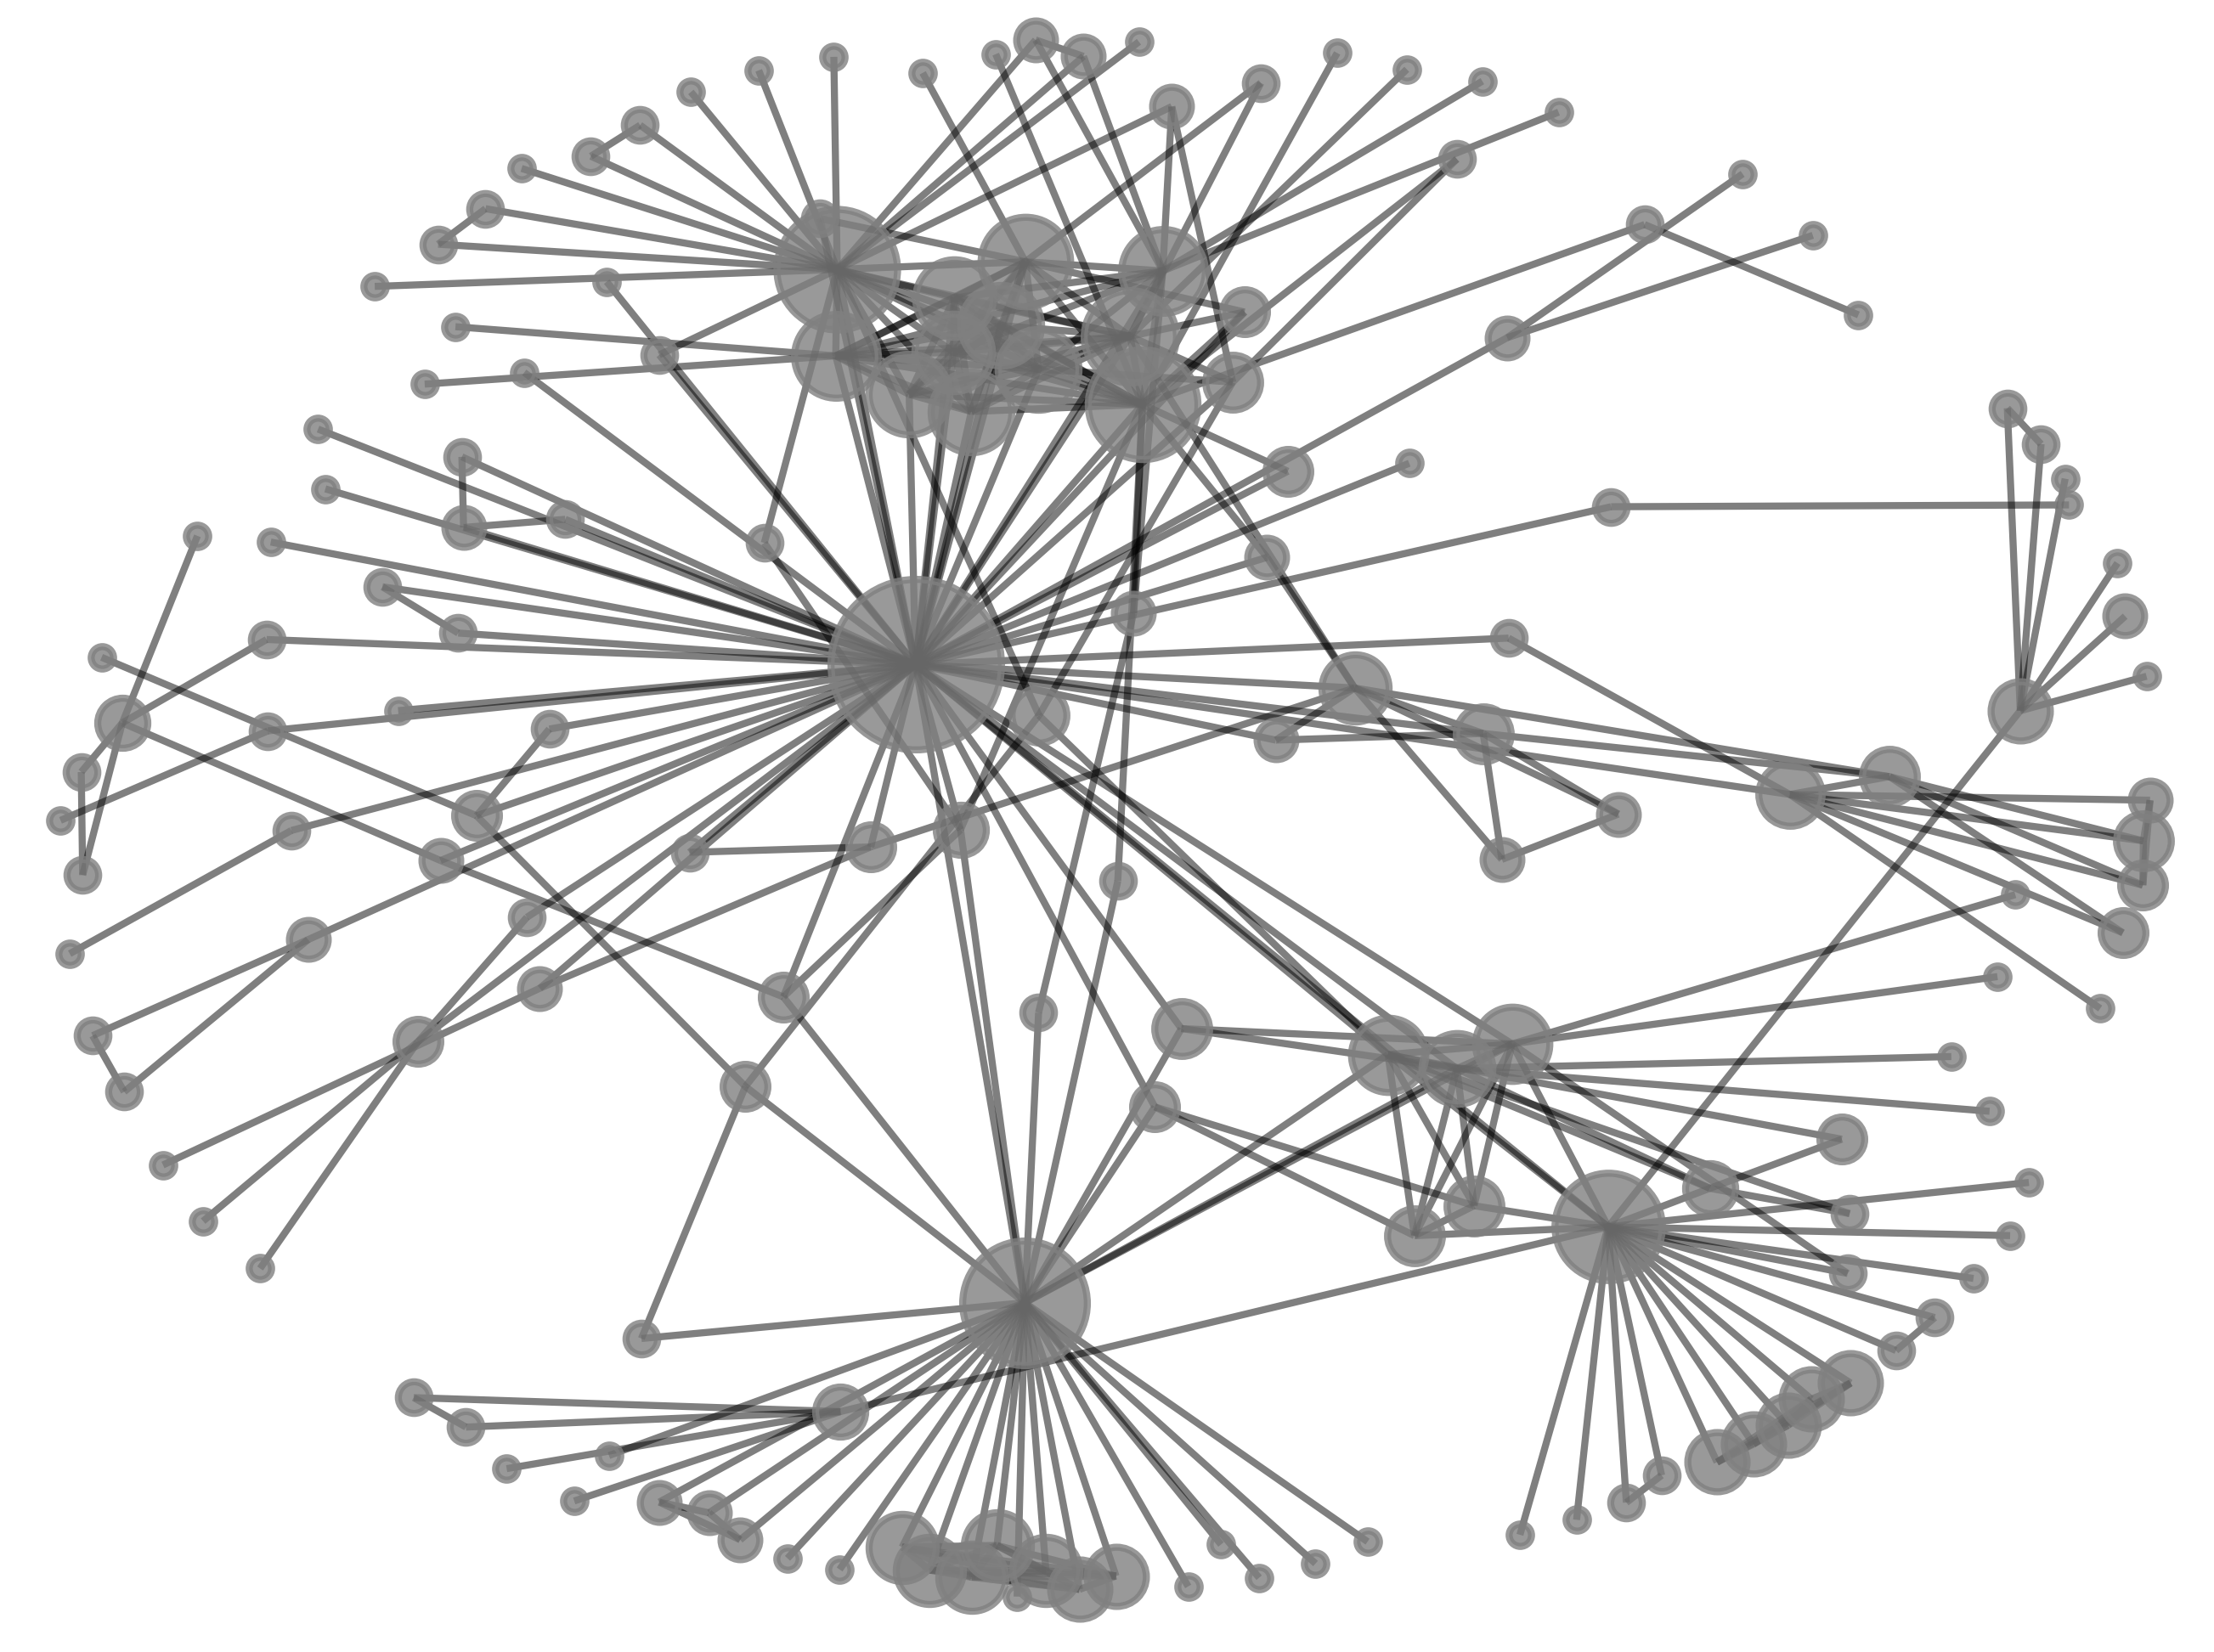
\includegraphics{OEIS/graph1}
\caption{Sequences network where vertices are emphasized according to the
number of incoming connections.}
\label{fig:oeis:sequences:network}
\end{figure}

\section*{Conclusions}

This chapter presents a suite of tools that interacts with the \textit{Online
Encyclopedia of Integer Sequences}, the primary goal is to automate simple and
repetitive operations such as (i)~crawling sequences to hold a local copy stored
in json format, (ii)~pretty printing data with filtering capabilities, both
in the terminal and in Jupyter (\url{http://jupyter.org/}) notebooks and,
finally, (iii)~to represent connections among sequences in graphs.

A further direction is to make graphs interactive, namely to tie together the
crawler and the grapher in a web-browser interface that when a vertex is
clicked it starts the fetching process, if it isn't downloaded already, and its
connections are added to the network dynamically.

\newpage
\begin{figure}
\begin{sideways}
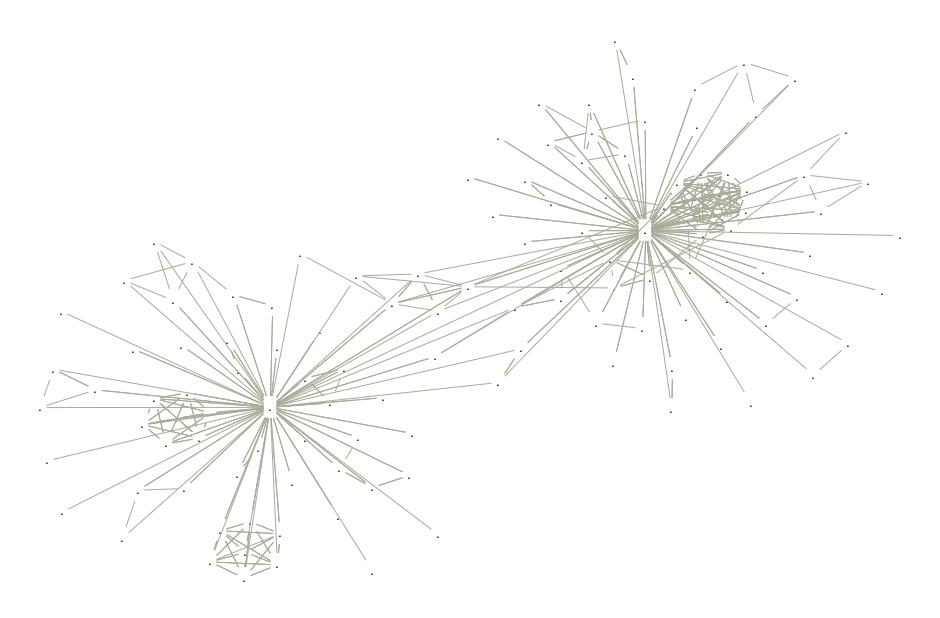
\includegraphics[width=20cm, height=30cm]{OEIS/points}
\caption{Sequences network abstracting over identifier to spot the underlying
structure.}
\end{sideways}
\label{fig:oeis:sequences:network:fibonacci:catalan}
\end{figure}

\newpage
\begin{figure}
\begin{sideways}
%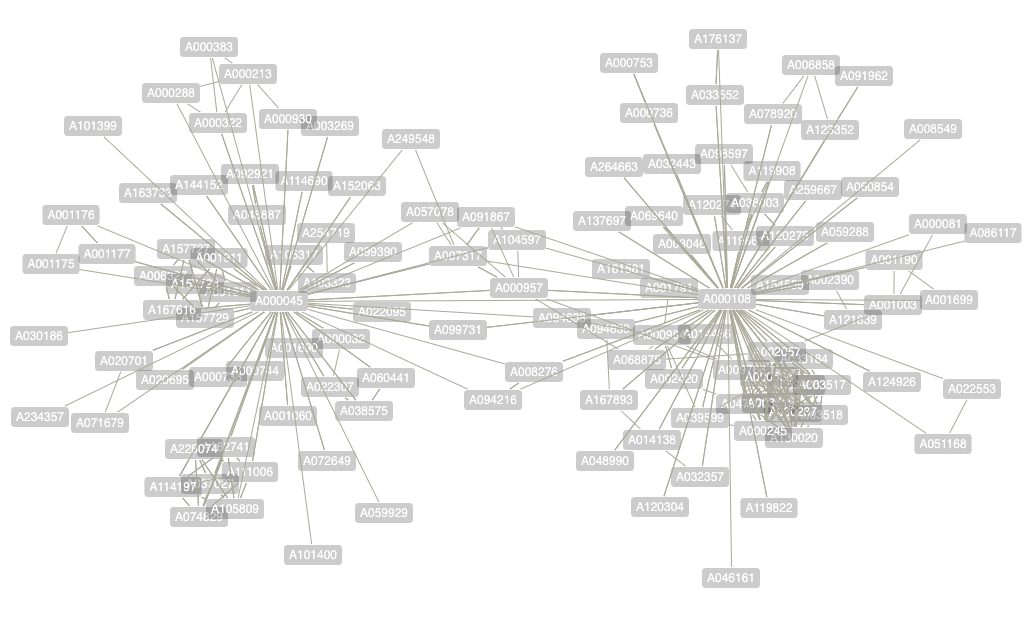
\includegraphics[width=20cm, height=20cm]{OEIS/labels}
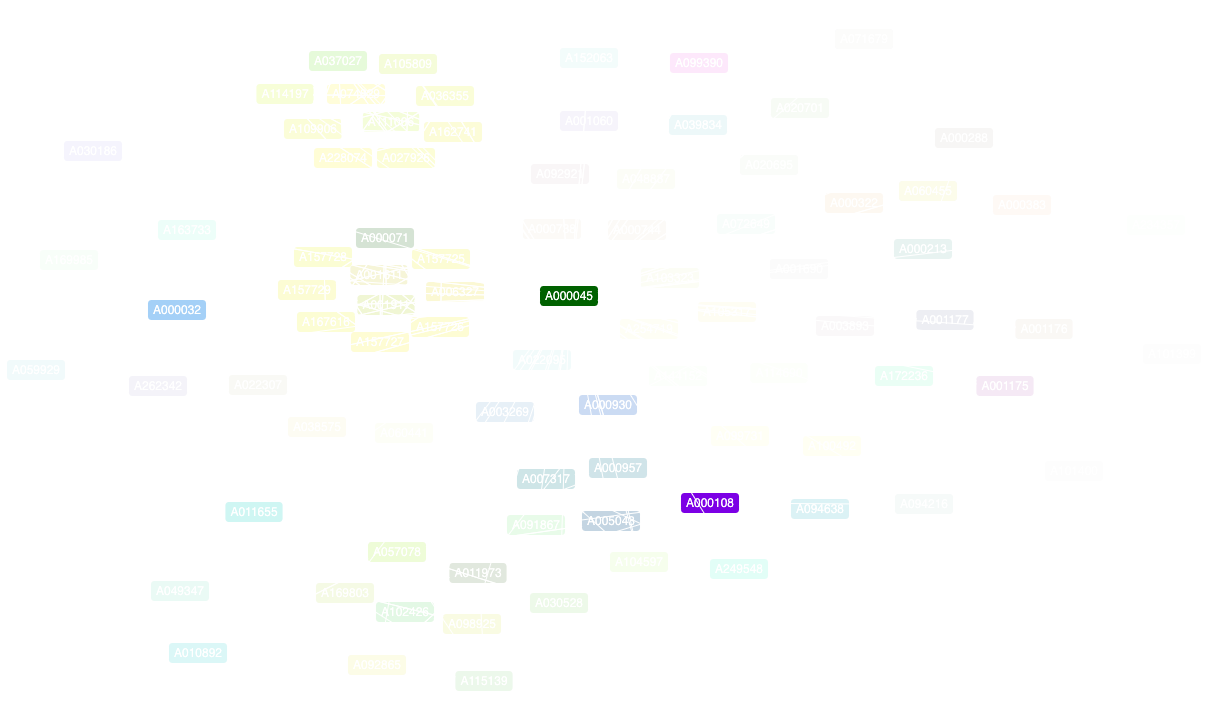
\includegraphics[width=25cm, height=25cm]{OEIS/coloured}
\caption{Sequences network with labelel vertices, here we see that the sequence
of \textit{Fibonacci numbers} (\url{https://oeis.org/A000045}) and of
\textit{Catalan numbers} (\url{https://oeis.org/A000108}) are the two central
sequences, respectively.}
\end{sideways}
\label{fig:oeis:sequences:network:fibonacci:catalan:labeled}
\end{figure}


\iffalse

\begin{figure}
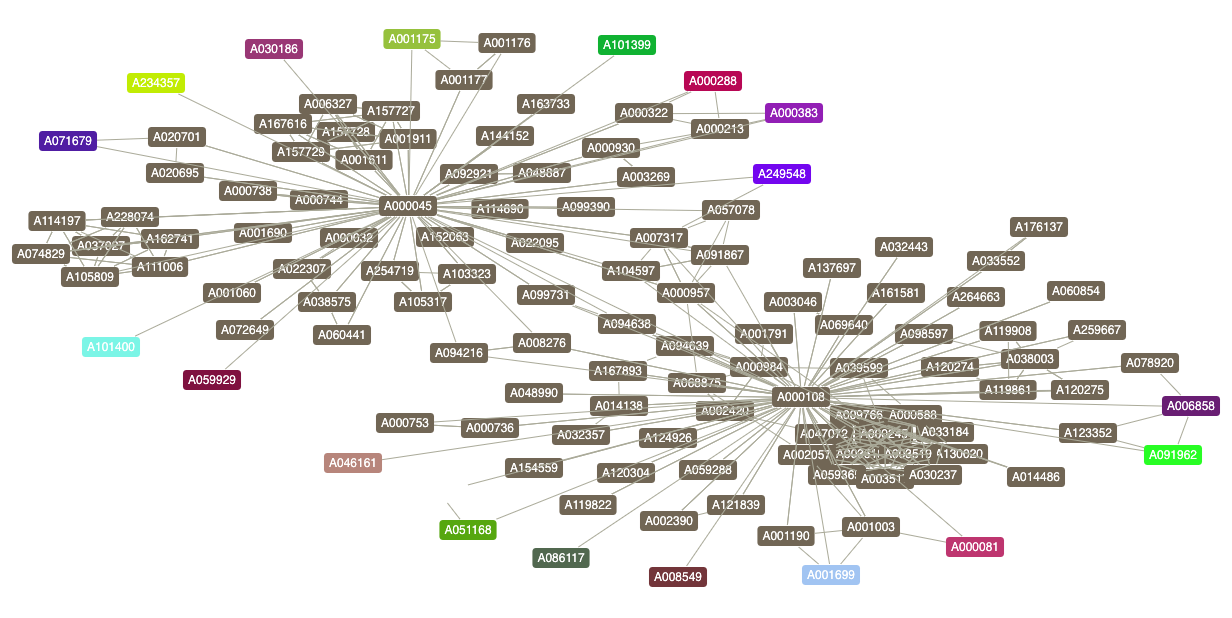
\includegraphics{OEIS/fibonacci-catalan}
\caption{Sequences network fetched by commands issued in the discussed session.}
\label{fig:oeis:sequences:network}
\end{figure}

\notbreakable{
    \inputminted[fontsize=\small,stripnl=false,firstline=31,lastline=44]
        {python}{deps/oeis-tools/src/graphing.py}
}

\notbreakable{
    \inputminted[fontsize=\small,stripnl=false,firstline=46,lastline=76]
        {python}{deps/oeis-tools/src/graphing.py}
}

\fi
